\documentclass[twoside]{article}

\usepackage{graphicx}
\usepackage[polish]{babel}
\usepackage[T1]{fontenc}
\usepackage[utf8]{inputenc}
\usepackage[table]{xcolor}
\usepackage{titlesec}
\usepackage{fancyhdr}
\usepackage[
    a4paper,
    inner=2.5cm,   
    outer=2.5cm,   
    top=2.5cm,     
    bottom=2.5cm,  
    footskip=1cm,  
    headheight=15pt 
]{geometry}





\definecolor{mojkolor}{RGB}{45, 45, 100}

\pagestyle{fancy}
\fancyhf{} % Wyczyszczenie domyślnych ustawień
\fancyhead[LE]{Aproksymacja Wielomianowa}
\fancyhead[LO]{Artur Radwański - grupa 4} % Lewa strona nagłówka
\fancyhead[R]{\thepage} % Prawa strona nagłówka
\renewcommand{\headrulewidth}{0.4pt}

\titleformat{\section}
  {\normalfont\Large\bfseries\color{mojkolor}} % Styl pisma
  {\thesection}                               % Numeracja
  {1em}                                       % Odstęp
  {}                                          % Tekst przed tytułem
  [{\color{mojkolor}\titlerule[1.5pt]}]       % KRESKA PO TYTULE (bezpieczna metoda)

% Dodatkowy odstęp pod kreską, żeby tekst nie "przyklejał" się do niej
\titlespacing*{\section}{0pt}{3.5ex plus 1ex minus .2ex}{2.3ex plus .2ex}

\begin{document}
\begin{titlepage}
\centering
\Large
\vspace*{1cm}
\begin{Huge}
 \textbf{Laboratorium Metod Obliczeniowych w Nauce i Technice - ćwiczenie 4a}
\end{Huge}


\vspace{0.5cm}
Ćwiczenie 4a - Aproksymacja Wielomianowa
            
 \vspace{1.5cm}

\begin{LARGE}
\textbf{Autor:}
\end{LARGE}
Artur Radwański



\vfill
            
Kraków\\ Semestr letni 2026

            
\vspace{0.8cm}

 
\includegraphics[width=0.4\textwidth]{agh.png}
            
Wydział Informatyki\\
Akademia Górniczo-Hutnicza\\


\end{titlepage}

\section{System}
\begin{itemize}
    \item Procesor: AMD Ryzen 7 9800x3d
    \item System operacyjny: 6.19.9-arch1-1 (Linux)
    \item Język programowania: c++23
    \item Kompilator: gcc version 15.2.1 20260209 (GCC) 
\end{itemize}

\section{Zadanie}
Celem zadania było zbadanie jak liczebność układu funkcji bazowych oraz zmienna liczba punktów dyskretyzacji wpływa na jakość aproksymacji. Badania przeprowadzono
dla przykładowej funkcji.
\begin{equation}
f(x) = -2x\sin(2(x-1))\hspace{5ex}  x\in[-2\pi+1,3\pi+1]
\end{equation}

\subsection{Model aproksymacji}
Wyznaczony wielomian aproksymacyjny $P_m(x)$ stopnia $m$ definiuje się jako kombinację liniową wielomianów Czebyszewa pierwszego rodzaju $T_i(x)$:

\begin{equation}
P_m(x) = \frac{1}{2}c_0 + \sum_{i=1}^{m} c_i T_i(\hat{x})
\end{equation}

gdzie $\hat{x} \in [-1, 1]$ jest wartością argumentu $x$ poddaną transformacji liniowej z przedziału $[a, b]$ według wzoru:

\begin{equation}
\hat{x} = \frac{2x - (a+b)}{b-a}
\end{equation}


macierz układu równań normalnych staje się diagonalna, co pozwala na optymalniejsze i bardziej stabilne numerycznie znalezienie
wzoru w porównaniu do metody gaussa.

\begin{equation}
b_k = c_k + 2\hat{x}b_{k+1} - b_{k+2}
\end{equation}

przy warunkach początkowych $b_{m+1} = b_{m+2} = 0$. Wynik końcowy obliczany jest jako:
\begin{equation}
P_m(x) = c_0 + \hat{x}b_1 - b_2
\end{equation}

\subsection{Metodyka pomiaru błędu}
Dokładność modeli została zweryfikowana na gęstej siatce $N = 10\,000$ równoodległych punktów testowych. W każdym punkcie wyznaczono błąd bezwzględny $\varepsilon_i = |f(x_i) - P_m(x_i)|$. Na podstawie tych danych obliczono:

\begin{itemize}
    \item \textbf{Błąd maksymalny ($E_{max}$)}:
    \begin{equation}
    E_{max} = \max_{1 \le i \le N} (\varepsilon_i)
    \end{equation}
    
    \item \textbf{Błąd średnikwadratowy ($\sigma$)}:
    \begin{equation}
    \sigma = \sqrt{\frac{\sum_{i=1}^{N}(\varepsilon_{i})}{N}}
    \end{equation}
    gdzie $\bar{\varepsilon}$ to średnia wartość błędu bezwzględnego.
\end{itemize}

Badania przeprowadzono dla różnych kombinacji liczby węzłów $n$ oraz stopnia wielomianu $m$, 
co pozwoliło na analizę zbieżności metody.

\section{Wyniki}
\input{tabelka.csv}
\input{tabelka1.csv}
\input{tabelka2.csv}
\input{tabelka3.csv}


Jak widać w tabelach \ref{tab:max} i \ref{tab:MSE} aproksymacja jest dokładniejsza wraz ze wzrostem liczby węzłów oraz stopniem wielomianu aproksymującego.
Zwiększanie liczby węzłów od pewnego momentu nie daje lepszych wyników dla tego samego stopnia wielomianu. Dzieje się tak, ponieważ aproksymacja jest
już bardzo blisko wielomianu danego stopnia który najlepiej ze wszystkich przybliża zadaną funkcję.

Odstępstwem od reguły jest aproksymacja stopnia 8 dla 10 węzłów. Jak widać na rysunku \ref{fig:unicorn} jest to kwestia niefortunnego ułożeni węzłów 5 i 6
która powoduje, że wielomian rośnie i osiąga maximum, tam gdzie funkcja zaczyna maleć i osiąga minimum. 

W tabelach \ref{tab:numerical_stability} i \ref{tab:super_numerical_stability} możemy zobaczyć, że metoda jest bardzo dobrze uwarunkowana i nie pojawiają się
znaczące błędy numeryczne nawet dla wielomianów rzędu kilkaset.

\begin{figure}
    \centering
    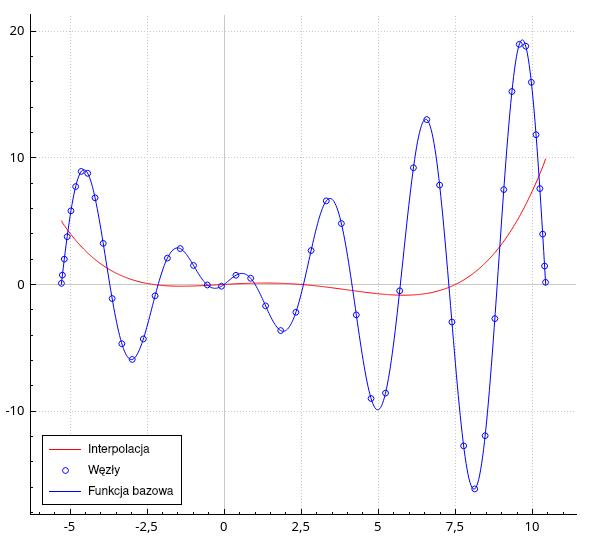
\includegraphics{wykres.png}
    \caption{m=8 n=10}
    \label{fig:unicorn}
\end{figure}
\end{document}